\documentclass{article}
\usepackage[utf8]{inputenc}
\usepackage{booktabs}
\usepackage{hyperref}
\usepackage{xspace}
\usepackage{graphicx}

\title{Scriptless Idle Modron Briv Farming}
\author{Hogo}
\date{July 2022}

\graphicspath{
{./images/}
{./images/champions}
{./images/sevenJumps}
{./images/sevenJumps/formation1}
}


\begin{document}


\maketitle
\tableofcontents

\newcommand{\separatingLine}{  
    \addlinespace[2pt]
    \hline
    \addlinespace[2pt]
}



\newcommand{\championMiniature}[1]{\includegraphics[width=8px]{#1}}

%add champion inlined image https://tex.stackexchange.com/questions/374192/how-to-use-figures-as-inline-images
%%%%% Characters
\newcommand{\artemis}{Artemis\xspace\championMiniature{artemis}\xspace}
\newcommand{\arkhan}{Arkhan\xspace\championMiniature{arkhan}\xspace}
\newcommand{\azaka}{Azaka\xspace\championMiniature{azaka}\xspace}
\newcommand{\blackViper}{Black Viper\xspace\championMiniature{blackViper}\xspace}
\newcommand{\briv}{Briv\xspace\championMiniature{briv}\xspace}
\newcommand{\baeloth}{Baeloth\xspace\championMiniature{baeloth}\xspace}
\newcommand{\celeste}{Celeste\xspace\championMiniature{celeste}\xspace}
\newcommand{\deekin}{Deekin\xspace\championMiniature{deekin}\xspace}
\newcommand{\desmond}{Desmond\xspace\championMiniature{desmond}\xspace}
\newcommand{\dragonbait}{Dragonbait\xspace\championMiniature{dragonbait}\xspace}
\newcommand{\havilar}{Havilar\xspace\championMiniature{havilar}\xspace}
\newcommand{\hewmaan}{Hew Maan\xspace\championMiniature{hewmaan}\xspace}
\newcommand{\jarlaxle}{Jarlaxle\xspace\championMiniature{jarlaxle}\xspace}
\newcommand{\melf}{Melf\xspace\championMiniature{melf}\xspace}
\newcommand{\minsc}{Minsc\xspace\championMiniature{minsc}\xspace}
\newcommand{\nayeli}{Nayeli\xspace\championMiniature{nayeli}\xspace}
\newcommand{\nahara}{Nahara\xspace\championMiniature{nahara}\xspace}
\newcommand{\nerys}{Nerys\xspace\championMiniature{nerys}\xspace}
\newcommand{\rust}{Rust\xspace\championMiniature{rust}\xspace}
\newcommand{\selise}{Selise\xspace\championMiniature{selise}\xspace}
\newcommand{\sentry}{Sentry\xspace\championMiniature{sentry}\xspace}
\newcommand{\shandie}{Shandie\xspace\championMiniature{shandie}\xspace}
\newcommand{\tyril}{Tyril\xspace\championMiniature{tyril}\xspace}
\newcommand{\yorven}{Yorven\xspace\championMiniature{yorven}\xspace}
\newcommand{\walnut}{Walnut\xspace\championMiniature{walnut}\xspace}
\newcommand{\widdle}{Widdle\xspace\championMiniature{widdle}\xspace}
\newcommand{\zorbu}{Zorbu\xspace\championMiniature{zorbu}\xspace}



%%%%% Patrons
\newcommand{\vjara}{Vjara\xspace}

\section{Disclaimer}

This is a work in progress.
I work on it when I find the time and or feel like it.
You may notice that there are a lot of placeholders for now.
Particularly, I am yet to add pictures.
This is planned, it's just easier to add a lot of text first.

If you have remarks on things that are \textbf{already} typed in, please feel free to comment on it in the modron \briv thread on the Idle champion discord (links will be added someday) Or wisp me on Discord directly: hogo\#8547.
You can also suggest some more placeholders section I will write in the future !
I also try to give credit whenever I remember about it.
Please tell me if I miss some, or give me the link to a message if I haven't tracked it down yet.
If you're polite and nice, I usually am nice too :)

Enjoy your read !

\section{Introduction}

Using Modron briv farming is an advanced technique use to idle gem farm in Idle champion more efficiently.
This guide is  an improvement on  \href{https://www.reddit.com/r/idlechampions/comments/rbldh0/automated_briv_stacking_without_scripting/}{Zeke's guide} hopefully clearing some things up, and adding some knowledge over this technique that we learn by discussing this on the discord (todoref).

It looks to use \textbf{\briv} which is the single most powerful speed champion in the game at this time.
\briv is able to jump over one or many areas thanks to his \textbf{unnatural haste} ability.

This technique is \textbf{scriptless} and only uses the game mechanics defined by developers.
Compared to script gem farming we have
\begin{itemize}
    \item More constraints (Only one formation, no script clicks, no offline stacking [...]);
    \item More lag (Because we require more champions, cannot clear memory leak with resets [...]);
    \item Less profitability;
    \item more set up difficulties. 
\end{itemize}
Then why use it you may ask?
I've seen some people say it's because they don't like scripting, some people have issue with the scripting tools, and many other reasons.
Mine is that I like the challenge of setting this up !


This is not a plug and play guide.
This is an advance guide that aims at covering as much concepts as possible so you can understand this technique in depth, and set up your own as you wish to do.
And even contribute later !
It is heavily dependent on your favors, champions, gears and multiple others.
You need to understand it in order to set it up.
I only give you the most important information here, but you have to do understand it in order to set it up.
If you do not understand it, it means this guide may be improved, so let me know !
Moreover, it might be a bit intimidating at first.
But don't loose hope !
Once you get it, you'll be able to set up anywhere you'll like !


\section{Definitions}

I start here by giving you some definitions that will ease the comprehension of the technique.
Particularly, I set the definitions of multiple Idle Champion defined concepts as well as adding a few of ours.

\subsection{Idle Champion Reminder}

\paragraph{Campaign.}
A campaign is a group of multiple adventure.
There are permanent campaigns and non permanent ones such as events todoref Wiki campaigns.

todoexample

\paragraph{Adventure.}

An adventure is a part of a campaign.
They are selected from the world map.
It also contains variants.

todoexample

\paragraph{Area.}

An \textbf{Area} is a map on which your character fight.
It's part of an adventure.
It's a zone between 1 and 50.
For example Area one is represented in \textbf{Zone}s 1, 51, 101, 151 [...].

todo example
\paragraph{Zones.}
A \textbf{Zone} is the current stage your party is fighting.
It's a zone multiplied by fifty.
A \textbf{Zone} uses an area and adds scaling information on the area.
Talking about a Zone is often done by using the "z" character before a number.
z51 = Zone 51.

\paragraph{Base Ultimate Damage (BUD).}

BUD is the highest damage that was set by a champion.
It is used to compute the damages of champion's ultimate damages, and firebreath potions.
More importantly it is the best visualization of your current damages.


\paragraph{Overwhelm}

//todo

\subsection{Advanced Concepts}

\paragraph{Gem Per Hours}

Metric used by Byteglow and Scripters to compare the efficiency of setups.

\paragraph{Boss Per Hours (BPH).}

Metric used by Byteglow and Scripters to compare the efficiency of setups.
This is a better measure of comparison than GPH because it varies less.


\paragraph{Potion Efficiency}

\textbf{Potion efficiency} means "how much of this potion am I using?".
This is particularly important for speed potions, as the others are generatlly not used for most of the run.
The ideal efficiency is to use as much as the possible potion time.
For example, using a small potion is 5 minutes.
If I use a small potion for a 1 minute reset, I use 20\% of my potion, this is not so good.
If I use a small potion for a 10 minute reset, I use 100\% of my potion, this is good because we profit from it all the time.



\paragraph{Potion Sustain}

Potion Sustain means "If I use a potion on every run, how long until I run out?".
Sustaining potions is difficult (Section \ref{sec:potionSustain}).
You do not have to sustain your potions all of the time.
Just remember that if it's a requirement for you (particularly for health potions), your setup will end up breaking.


\paragraph{Perfect Jumps.}

\briv chances to jump over the next N areas.
This chances are regulated by \briv 4th item slot.
Perfect jumps are when \briv has 100\% chance of skipping the next N area.
The item level required to be perfect jumps are computable with multiple tools.
Particularly I personally use the great Byteglow online tool todoref.
This technique is significantly easier to use with a perfect jump. 

\paragraph{Quick Transition (QT)}

Usually, when the party finishes the zone's requirement, it walks over to the next area.
A \textbf{Quick Transition} is a transition between two zones in which the party does not move.
This is \textbf{significantly} faster for gem farm.
The main adventures that exhibit  \textbf{Quick Transition}s are \textit{Tall Tale} (TT) and \textit{The Everlasting Rime} (ER).
They are of course other adventures that exhibit QTs, but they are less popular since they have less \textbf{Quick Transition}s (Picture).
Moreover, a \textbf{Quick Transition} depends on the number of jumps (picture)
I also developed a query-able database of the adventure of Idle Champion that allows anyone to compute the \textbf{Quick Transition}s for any adventure \footnote{I'm the only use so it's rought for now. \url{https://github.com/hogoww/IdleChampionTooling}} based on Kleho's website \footnote{\url{idle.kleho.ru/}}.
This allows me to quickly compute any QTs for a given adventure (Table~\ref{tbl:tallTaleQts} or to find out which adventure has the most QTs for a given jump (Table~\ref{tbl:fourJumpsQts}).

\paragraph{Zone Loop.}
The \textbf{Zone loop} is the number of zones you need to clear in order to be back to the area where you started.
A few illustrative example.
I'm starting z1.
If I have 0 jumps, I will encounter this area again at z51.
If I have 4 jumps, I will encounter this area again at z51.
If I have 7 jumps, I will encounter this area again at z201.


\begin{table}[ht!]
\centering
\caption{Number of QTs for the The Everlasting Rime aventure, depending on the number of jumps.
For example, If I have 2 jumps, 48\% of the transitions are QTs.
}
\label{tbl:tallTaleQts}
\begin{small}
\begin{tabular}{ c | c }
\toprule
Number of jump & number of QTs \\
\midrule
0 & 54\% \\
1 & 52\% \\
2 & 48\% \\
3 & 48\% \\
4 & 50\% \\
5 & 44\% \\
6 & 42\% \\
7 & 40\% \\
8 & 38\% \\
9 & 40\% \\
10 & 34\% \\
11 & 32\% \\
12 & 30\% \\
13 & 28\% \\
14 & 30\% \\
\bottomrule
\end{tabular}
\end{small}
\end{table}

\begin{table}[ht!]
\centering
\caption{Number of QTs per adventures for 4 jumps \briv.
}
\label{tbl:fourJumpsQts}
\begin{small}
\begin{tabular}{ l c c }
\toprule
Campaign & Adventure & Number of QTs \\
\midrule
Witchlight & Tall Tales & 60\% \\
Rime of the Frostmaiden & The Everlasting Rime & 50\% \\
Witchlight & The Firy Rings of Thither & 30\% \\
Descent into Avernus & The Path of Dreams 30\% \\
Descent into Avernus & Resolve Amongst Chaos & 30\% \\
Descent into Avernus & The Bleeding Citadel & 30\% \\
Grand Tour & Excavating History & 30\% \\
Grand Tour & Towering expectation & 30\% \\
Witchlight & Slack-jawed Lorna & 20\% \\
Rime of the Frostmaiden & Ending the Rime - Part 1 & 20\% \\
\bottomrule
\end{tabular}
\end{small}
\end{table}

\subsection{Guide specific.}

\subsubsection{Concepts}

\paragraph{Click Wall.}

Click damage is upgradable.
Your click damage is therefore able to kill monsters.
It even one shot monsters with high enough upgrades in it !
We call \textbf{Click Wall} the zone in which the click damage is not able to one shot monsters anymore.
Click damages might still be to clear your \textbf{Click Wall} zone, but it's still your \textbf{Click Wall}.

It is roughly calculated by taking the power of your favor (enable scientific notation) and multiply it by 7.43.
For example, I have 5e100, my click wall is around zone $100 * 7.43 = 743$ !

\paragraph{Stacking Zone (= Hard Wall).}

The \textbf{Stacking Zone} is the zone in which neither the click damage nor the champions are able to kill anything.
In regular play, it's the maximum zone reachable with all the tricks you are able to think of.
In this guide, it's a zone on which your click damage are not able to kill anything anymore, in spite of the click wall extender champion (Section~\ref{sec:clickWallExtender}).

\paragraph{Zone Spread.}

The \textbf{Zone Spread} is the number of areas between your Click Wall and your Hard Wall.
It allows you to loose click damage until a point in which the click damage is not able to kill anything anymore.
%Need to find correct credit.
Calculated by NNN(find credit), you need a \textbf{Zone Spread} of at least 17 areas to loose enough click damage to not kill anything on your hard wall.

\subsubsection{Champion Jobs}

\paragraph{Click Wall Extender.}
\label{sec:clickWallExtender}

The \textbf{Click Wall Extender} is a character (or more) that increases the click damages.
Having a \textbf{Click Wall Extender} allows to go from the Click Wall to the Hard Wall as fast as possible !
There are multiple champions possible for the jobs.
Particularly, \minsc is allows click damage to be increased against a kinds of enemies out of 5.
A list is available in Section~\ref{sec:stepTwo}.

\paragraph{Trigger Champion.}

A \textbf{Trigger Champion} is a champion that gives a boost of damage from some event.
In Zeke's guide for example, it's \dragonbait.
When the creep enrage, \dragonbait provides an additional damage buff.

\paragraph{BUD Setter.}

The \textbf{BUD Setter} is the champion that hits the hardest and sets the BUD.
It's usually the most buffed damage dealer.


\section{Using Modron Briv Stacking}

\subsection{Requirements}

The following are required:
\begin{itemize}
    \item A modron core with automation available;
    \item A \briv with at least 1.2 jumps (ref zeke);
    \item A trigger champion;
    \item Adequate favor;
    \item Adequate adventure.
    \item 5 clickers for the most simple setup Ideally, we need 17 clickers.
\end{itemize}

Optional (but pretty nice !):
\begin{itemize}
    \item Other champions improving Speed other than \briv (see Section \ref{sec:stepFour}).
    Recommended: \widdle (2), \shandie (6) and \hewmaan (8).
    Optional: \deekin (1), \nahara (3) and \sentry (4), 
    \item A Click Wall Extender
\end{itemize}
 


\subsection{General Concept}

Beware: this technique is \textbf{significantly more difficult} to set up for non-perfect jump.
I advise to stay at perfect jumps starting at 3 jumps.
Only put contracts when you have enough to go the next perfect jump chance (Section \ref{sec:upgradeIlvl}).
Moreover, even if you are using a non-perfect jump \briv (Section \ref{sec:nonPerfectJumps}), I'd advise to look at the part for perfect jumps first, as it is probably easier to understand.

The gem farm goes about as such:
\begin{itemize}
    \item Clicker kill everything until the click wall;
    \item Clicker or champion kill mobs until the stacking zone (Section~\ref{sec:stepOne});
    \item The party arrives to the stacking zone nobody kills anything(Section~\ref{sec:stepTwo});
    \item \briv tanks and re-stacks for the next run (Section~\ref{sec:stepThree});
    \item When \briv has enough stacks, the party kills everything thanks to the trigger champion (Section~\ref{sec:stepFour});
    \item Restart (Section~\ref{sec:stepFive})!
\end{itemize}

Each of these steps is described further in the following.

\subsubsection{Step One: choose Your Target}
\label{sec:stepOne}

Any zone can be a target.
For example, I once set this technique up to farm \briv chests during his event.
However, the ideal properties are a zone on which you are able to use a Click Wall Extender.
Usually, multiple zones in a row need to have a certain property.

\begin{description}
    \item[\minsc.] (Slot 7) \minsc adds damages against a certain kind of enemy with the ability \textit{Favored Enemy}.
    Moreover, it also adds damage to the Click damage !
    Possible types are: Human, Beast, Undead, Fey and Monstrosities.
    Moreover this is buffed by \minsc 4th item.
    Therefore it adds a lot more damage than others champions against those targets !
    This is the most used champion to use as a click wall extender.
    This is also the only one represented in the table, because it's the one that got the most feedback on, and the one I personally use.
    \item[\zorbu] (Slot 12) \zorbu's \textit{Lifelong Enemy} increases the damages against Humain, Beast, Undead and Drow.
    However this does \textbf{NOT} apply on click damages, nor does it apply on other champions.
    Therefore using \zorbu as a click wall extender does not work.
    However, he does more damage against this kind of enemies.
    Therefore, if he is the BUD setter, he smooths the transitions toward the stacking area in the same manner a click wall extender does.
    \item[\azaka] (Slot 12) \azaka has a debuff that increases the champions damages when fighting outdoor.
    Therefore the transition from the click wall to the stacking zone may work if you find an adventure on which your jumps get from outdoor to indoor, with the required zone spread.
    \item[\nerys] (Slot 12) \nerys has a small debuff against undeads that does not scale, but seem to apply on click damage.
    This can help if you have a small zone spread before Minsc kicks in, for example.
\end{description}

Others may be a good fit, but are not as good as the ones described here.

The stacking area should be a non boss area.
Range enemies have been shown to give more stacks for the same amount of time and damages in the zones we used.


\subsubsection{Step Two: Tune Click Damage}
\label{sec:stepTwo}

To tune your click damage, you have to tweak the gold find.
The main source of gold find is favor.
I always recommend to shoot just bellow the point that you need, to be able to tune it with other methods.
Particularly, a level 15 speed core provides up to e4.5 gold find //tocheck.
To compute the required favor, divide the target area with the magic number 7.43.
For example, I want to stack at z691 on Tall Tales.
For that purpose, I look up in the Table \ref{tbl:adventures}, the click wall should be at the lowest at 656.
$656 / 7.43 = 88$, therefore I need to farm e88 favor.
As I said before, I tend to aim a bit lower to be able to tweak it if needed.
In this case, I would go to e85 and add modron nodes.

To get more Gold find, you may:
\begin{itemize}
    \item Farm favor;
    \item Add modron gold find nodes;
    \item Champions.
    The main champion you may use are \rust, \jarlaxle and \azaka.
    They are the most consistant gold find providers.
    Particularly Rust, because he won't get more item level from opening silver and gold chests.
\end{itemize}

Note that the click damage should be at least e3, ideally even e4 lower than the stacking zone monster's health.

\subsubsection{Step Three: Tune Briv's Stacking}
\label{sec:stepThree}

To get stacks, \briv must tank attacks from enemies.
You therefore have to clear the area only after you get enough stacks, otherwise you will not be able to jump all the way back to your stacking zone.


Once you have a stacking zone in mind, you may compute how many sprint stacks you need to reach it.
Byteglow has a great calculator to compute the number of stacks you need.
Remember that the more area you want to jump over, the more stacks are needed to jump over just one zone.
The rule of thumb I usually follow is to aim lower than 6000 stacks, after that it's taking too much time.
3000 to 5000 stacks are usually the higher range you want to aim at.
Under 3000 is usually fairly easy.


Having too little to no stacks will slow down the farm terribly.
For perfect jumps:
    Overstacking does not matter in the slightest.
    Understacking prevents you to jump to your stacking zone, preventing you to get enough stacks for the next run.

For non perfect jumps:
    Overstacking may jump passed your stacking zone, leaving you with little to no stacks.
    Understacking allows you to ensure that you will be at least some kind of fast, and walk the lasts areas as expected.

First, do not concern yourself with damages.
Only look at how much health your \briv needs to get enough stacks.

To improve survivability:
\begin{description}
    \item[Feats] The best feat for \briv so far are the Overwhelm feats by far.
    The health feats, although tempting, do not compare.
    For other tanks, the health feat increases briv's health, hence they are the best in this case.
    \item[Mirtt's \textbf{Perk's Up}.] This perk, that increases tank's healing.
    \item[More health] there are multiple ways of increasing health.
        \begin{itemize}
            \item Most tanks have a health share ability.
            Moreover many tanks have a health scaling item.
            Therefore more tanks, more health.
            To have a tank provide health however, it requires to have some item level in their health item.
            This is why we often choose Evergreen champions that continuously scale up.
            Particularly, \dragonbait, \tyril and \nayeli.
            \tyril and \nayeli need to be in right specialization.
            \item Vjara and Zariel perks increase health moderately.
            \item Champion feats, particularly tanks.
            Careful, overwhelmed feats are better for \briv.
             \item Health potions.
            Beware of using Health Potions.
            You will not be able to sustain them for a long time (Section \ref{sec:potionSustain}).
            We empty our stocks more quickly than we think.
            Note that the more tanks are used, the more health the potions are bringing.
        \end{itemize}
    \item[\baeloth's djinn.] \baeloth's djinn ability gives 30 second of invincibility upon death.
    \item[Damage reduction.] This is currently not viable.
    \begin{description}
    \item[\yorven.]
    \yorven reduces the damage taken by adjacent champions by a small amount.
    However \yorven puts a debuff on a single enemy on each attack.
    This debuff increases the click damages, making tuning your click damage more difficult (Section~\ref{sec:stepTwo} and Section~\ref{sec:stepFour})
    Similarly, this debuff increases the damages of champions, making tuning of your BUD more difficult (Section~\ref{sec:stepFour}).
    \item[\selise] 
    \selise reduces the damage taken from melee while in \textbf{wall stance} for the champions in her column.
    However you need use the ultimate once to get into \textbf{wall stance}.
    Moreover, while in \textit{aggressive stance}, the default stance, she stuns enemies, reducing the number of stacks you'd get.
    Finally, the placement requirement is just not viable most of the time because of Hew's requirements.
    \end{description}
    \item[Healing.]
    Every healing ability (besides \briv's) is around a fixed e4 health.
    However very quickly briv gets e7+ health (by just adding \dragonbait in).
    Therefore, it's mostly useless.
    A few ultimates attacks are healing massively, namely \celeste, \widdle and \walnut but none of them are viable in a gem farming setup.
\end{description}



\subsubsection{Step Four: Tune Your BUD}
\label{sec:stepFour}

Once you know at what time your stacks are high enough, you can prepare your BUD.
You should use a trigger champion that buffs your BUD setter.
But first, let's add some speed !

\paragraph{Party size and lag}

Before you start know that adding a champions adds code behavior, image rendering and many things.
Therefore it adds lag.
If you can remove a character or a pet at some point

\paragraph{Speed champions first !}

Before actually working on the BUD, it's time to add speed champions !
You either consider them as mandatory for your purpose (shandie for example), or if it is possible (such as Sentry).
You will have to manage with those constraints.
Usually we consider that if a slot can stay empty, that's better than a character that adds too little benefit.



\begin{description}
    \item[\deekin.] (1) \deekin is a very good plug and play champion.
    Put him anywhere and enjoy !
    He increases the speed of enemy pop.
    The specialization is \textit{Boss Wants Speed} (right).
    He is improved by a feat that is looted in gold chests.
    It is unaffected by his gear.
    Using \deekin and \widdle is redundant and usually should be avoided.
    Usually we consider that it is either \deekin OR \widdle.
    
    \item[\widdle.] (2)\widdle is usually considered to be better than \deekin.
    She should be next to as many champion as possible.
    I have read multiple time that once \widdle's \textit{Tasty Friends} has 1000\%, it's capped (I have not verified myself).
    She increases the speed of enemy pop.
    The specialization matters little, because she only exclude a few champion from each, and not many of them are relevant for gem farm.
    \textit{Tasty Friends} is buffed by \widdle 4th item.
    She has a Golden Epic, which seems to not be very useful from a speed standpoint as the cap is achieved quite easily.
    Using \deekin and \widdle is redundant and usually should be avoided.
    Usually we consider that it is either \deekin OR \widdle.
    
    \item[\nahara.] (3) \nahara reduces quests requirement as long as she \textit{should} kill enemies even though they die from clicks.
    Her placement imports little, but if you want to have as much benefit from her as possible, she should be your BUD setter.
    The specialization is \textit{A Skilled Lyre} (right).
    Her speed skill \textit{To Amuse or Avenge} is not affected by gear/feats at this time.
    Note: it can apparently become pretty laggy when you hit 100 enemies while stacking.
    Note2: see common note on quest requirement after this list.
    
    \item[\sentry] (4) \sentry reduces quest requirements if she wasn't hit by enemy on the previous area.
    Her placement does not change anything.
    The specialization is \textit{Echo's Will} (middle).
    \textit{Echo: Resolution} is buffed by \sentry 4th item.
    It has a cap at 100\% reduction, which you can compute on Byteglow.
    She has a golden epic for this item, that does not make much sense to buy as the cap is quite low already.
    Note: She is conflicting with Baeloth, so if you can use another trigger than baeloth, that's usually better !
    Note2: see common note on quest requirement after this list.
    
    \item[\shandie] (6) Probably the best plug and play champion.
    After a minute without any champion being attacked, \shandie increases the speed of the game.
    Her speed ability is not affected by her placement.
    %She buffs damages for the column in front of her with \textit{Explosive Arrow} depending on enemy hit by her attack as well as in a radius of two cases with \textit{Agile Allies}.
    %Usually I'd advise to not rely on \textit{Explosive Arrow}.
    %The number of enemy hit might be inconsistent, particularly when stacking on range enemies.
    Her speed ability \textit{Dash} is only affected by specialization \textit{Ranger Training} (left).
    
    \item[\hewmaan.] (8) \hewmaan is the second best speed champion, right after briv (even after the recent nerf).
    They increases the number of quest item looted and enemy kill counts.
    Their speed ability depends on their placement in the formation.
    \hewmaan.
    They should be in the front column in 3 and 4 column formation, or in the front two column in other formations.
    On top of that, \hewmaan has to be adjacent to as many champions as possible.
    The specialization is \textit{Carefully Balanced} (right).
    Their \textit{Teamwork} ability is buffed by the 4th item as well as very good feats.
    It is capped, check out Byteglow.
    Note: see common note on quest requirement after this list.
    \item[\havilar.] (10) This is currently broken.
    The developers have said they are considering adding this back in the future \footnote{Developer insights: \url{https://www.twitch.tv/videos/1538716891}.
    Community recap (thanks @J\_Dawg\_27!): \url{https://discord.com/channels/357247482247380994/357247483111276546/999801304639602718}}
    Out of \havilar's 4 imp, Dembo double the quest drop and kill counts from \textbf{imps} enemies.
    Therefore this does not work in every map, but it has its uses.
    Note: see common note on quest requirement after this list.
    \item[\melf.] (12) Considered to be worse than an empty spot by the scripting community.
    I trust them, and do not explain him further.
\end{description}

An additional speed feature that is not from a champion is the \textbf{Brisk Benefactor} Witchlight local blessing.
It reduces quest requirements (in Witchlight adventure) by 20\% while running the adventure with a patron.
That is pretty neat given that \vjara has constraints that works \textbf{very} well with usual speed gem farming !
The only downside is that you have to use the constitution feat for widdle.
This introduces well the note on quests requirements.

Note on quest requirement: Quests requirements reductions might not all be worth it at once.
For example \vjara + \nahara brings less benefit than only using one of them.
//TODO more detailed note
%tocheck
%Particularly, we've seen low interest in having \sentry and \nahara (Thanks to Primate's).

\paragraph{Choosing a trigger champion.}

I identify 3 kinds of possible triggers (there are a few more that do not look viable to me):
\begin{description}
    \item[Enemy count] There are a few champions that give damage boost depending on available enemy.
    For example, \shandie's explosive arrow.
    This gives a boost that may be enough.
    I found it to be the less consistent, and I usually try to \textbf{not} affect my BUD setter with explosive arrow.
    Moreover ranges enemies are scattered.
    Therefore the number of enemy may not be consistent.
    
    \item[Enrage stack count]
    After you get a 100 enemies in a non boss area, an enrage count starts.
    This is similar to bosses enrage count.
    Multiple tank champions buff the damages of champions depending on the number of enrage stacks.
    This is the case of \dragonbait, \tyril and \nayeli.
    Each stack of enrage gives a little bit more buff.
    
    \item[\briv death] At some point \briv should die due to the number of enrage stacks.
    \baeloth's trigger is the only one that has worked so far with \briv death (if someone wants to try out \desmond, give me feedback?).
    When \briv dies and \baeloth's Djinn trigger, a big amount of damage boost that should allow you to clear the area.
\end{description}

The trigger champion is often chosen by the reset level, and the damage \briv's is under ect.
For example, it's harder to use \briv death as a trigger at lower levels.
Similarly, using enemy count at high levels may not be appropriate because you need more stacks than the hundred enemy cap can provide.

A particular extra mention for debuffs.
In theory they could work.
However, since they interact with click damage, they are gonna be a pain to deal with.
I don't know of anyone who did work with them.
If someone figures out how to make it work, let me know please :)
I personally think that's not worth the pain.

\paragraph{Choosing a BUD setter}
BUD setter may be any character.
I even used \nerys at some point !

One property that I personally like in my BUD setters is to get amplify the trigger.
This is the case of \artemis, \arkhan (untested) or \blackViper (untested).
Personnally I used \artemis in every set up I do.
This is because he observe the trigger over multiple champions, and therefore benefits from an amplified effect.
However the jeweled power ability increase your next auto attack upon killing an enemy.
Therefore your first attack with \artemis on the stacking zone should never kill an enemy.

Another special mention is \nahara

\paragraph{Additional ways of tweaking the damages.}

\begin{description}
    \item[Blessing and Patron.] I usually do not deal with them, because I always forget to put them back when doing something else.
    \item[Modron core nodes.] this gives pretty big boosts, even more so now that overcharged is a thing;
    \item[Feats.] Feats are pretty minor compared with Modron core nodes, I usually keep them for final tweaks.
    I also try to not touch them too much, to allow different setups.
    \item[Support champions] duh.
\end{description}


\subsubsection{Step Five: Monitor}
\label{sec:stepFive}

It worked once !\newline
It will always work !\newline

No.\newline
Things are often inconsistent, particularly at the start.
We usually have to watch a bit to see how the farm is behaving.
Don't worry, you'll get a sense of when this will be inconsistent at some point.
Plus, monitoring does not mean looking all the time.
Just check whether it continues jumping from time to time !
It is always more important to look for consistency than squeezing a bit more performance out of your gem farm.
Always save your working setup before experimenting with another setup.

Things that may add inconsistency that we identified are:
\begin{description}
    \item[Lag.]
    The less champions and clickers you have, the less lag you are subject to.
    Less lag, more farm.
    More lag less farm, and inconsistencies.
    
    \item[Distractions.] Using a 6th clicker to kill distractions may give unexpected inputs of golds, which would give too much click damages.
    
    \item[Extra quest rewards.] Level 15th node in the speed core may give different gold inputs by ending some levels early.
    This is often not a problem for perfect jumps.
    
    \item[Using Ultimates] Using ultimates, particularly with clickers.
    They may end the run a bit early because the BUD is high enough for an ultimate to kill targets, but low enough that you are not at the expected stacks number yet.
    I used to be able to use ultimates without issues, but not anymore, not sure of why.
\end{description}


\subsubsection{Non-Perfect Jumps Particularity}
\label{sec:nonPerfectJumps}

todo

\subsection{Choosing an Adventure}

The first question we get asked is which adventure to target ?
How do I choose my adventure ?
If you are only interested in existing results, I provide a list we compiled with their click wall, stacking zones and other relevant information.
If you want to know how to choose an adventure, it's after the list !


\begin{table}[ht!]
\caption{Adventures for Modron \briv gem farming.
The general adventures are adventures that can be chosen for any kind of jump chances, perfect or not.
Particularly, we currently do not have a good adventure for 6 or 8 jumps \briv .
I also put Minsc specialization as this is the most common click wall extender.
}
\label{tbl:adventures}
\begin{small}
\begin{tabular}{ l | l c c c c }
\toprule
\textbf{Jumps} & \textbf{Campaign} & \textbf{Adventure} & \textbf{Click} & \textbf{Stacking} & \textbf{Favored}\\
&&&\textbf{Wall} & \textbf{Zone}& \textbf{Enemy}\\
\midrule
0       & Sword Coast  & Supply Run         & z5 & z19 & Beast \\
        &              & Terror In the Dark & z6 & z18 & Beast\\
        & Avernus      & todo & & &\\
\separatingLine
3       &  IWD & The Everlasting Rime (ER) & z61 & z97 & Beast\\
\separatingLine
4       &  IWD & The Everlasting Rime (ER) & z21 & z41 & Beast\\
        &  WhitchLight & Tall Tales (TT)   & z11 & z41 & Fey\\
\separatingLine
7       &  IWD & The Everlasting Rime (ER) & z57 & z97 & Beast \\
\separatingLine
9       & WhitchLight & Tall Tales (TT)    & z11 & z41 & Fey \\
\bottomrule
\end{tabular}
\end{small}
\end{table}

For each kind of jumps, I will detail further some detailed examples of setups.

\subsubsection{3 Jumps}

Everlasting Rime is Queen

\subsubsection{4 Jumps}

Tall Tale > Everlasting Rime > anything else, basically

\subsubsection{7 Jumps}

The Everlasting Rime is Queen.
It is the adventure with the most QTs for 7 jumps (50\%)
The main downside is that it has only one viable stacking and reset points, that is 200 areas apart.
The jump loop is 200 areas.
Therefore the two realistic points are stacking on 897 (1866 stacks) and 1097 (4206 stacks).
897 reset: Easier, better potion efficiency, better BPH.
1097 reset: Hard, better potion sustain.

With 7 jumps, you avoid the main problem of The Everlasting Rime which is the z50 boss, which almost always breaks \shandie's dash.
Finally, minor annoyances are barricades (z193) and 3 hit based health (z33).


\paragraph{A first 1097 stacking}

/!\\ Not potion sustainable /!\\.

Gold find: 2e138\newline
Favor: 5e133\newline
Formation: Figure~\ref{fig:sevenJumpsFormation1}\newline
Click Wall: 1057\newline
Stacking Zone: z1097\newline
Resetting: z1098\newline
BUD required: e337\newline
Briv health required: Around 5e10 (Still the required values)\newline
Click Wall Extender: Minsc (beast)\newline
Trigger Champion: Baeloth\newline
BUD Setter: Artemis (about 6k ilvl)\newline
Legendary Gear Bonus: 7.97e40\% damages\newline
Core: Fast Core 1.62e24\% damages\newline
Potions: Speed (small 1 + medium 1) Health (small 993 + medium 993 + large 1)

Details:
It was quite tricky to have enough survivability, and enough damages.
I also had no space for additional gold find champions while my favor was too low.
So far I couldn't use \widdle, I do not have the damages.
Similarly, I had to have \tyril.
This setup is not sustainable because I need large health potions to have enough health to survive long enough to stack.
Which is not sustainable.

\begin{figure}[h]
    \centering
    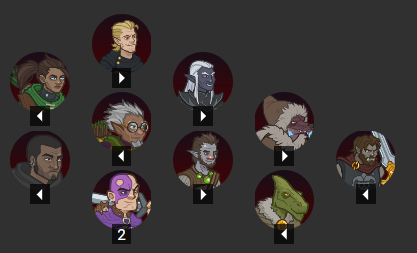
\includegraphics[width=\linewidth]{sevenJumpsFormation1}
    \caption{Basic formation for a first z1097 farming.}%
    \label{fig:sevenJumpsFormation1}
\end{figure}

\subsubsection{9 Jumps}

Back to the great Tall Tale adventure

\subsubsection{Specific Adventure Set Up}


sevenJumpsFormation1

\subsection{Champion Roles}

Todo list of champions and their possible roles

%%%%%%%%%%%%%%%%%%%%%%%%%%%%%%%%%%%%%%%%%%%%%%%%%%%%%%%%%%%%%%%%%%%%%%%%%%%%%%%%%%%%


\section{Tips And Tricks}

\subsection{Extra Free Gems}

For perfect jumps only.

If after your stacking zone, you have enough for one more jump, you can reset a zN+1.
For example in ER, you can reset at z42 rather than z41.
The jump will effectively happen, making the party go to z46.
This will award you the z45 gem bag for free.

You should always reset at z42 rather than z45 though, because if for some reason you understack and do not have enough for this extra jump, you will only have to clear one area rather than 4.

%%%%%%%%%%%%%%%%%%%%%%%%%%%%%%%%%%%%%%%%%%%%%%%%%%%%%%%%%%%%%%%%%%%%%%%%


\section{Frequently Asked Questions}




\subsection{Dealing With Favors Too High}

If you have too high favor, you have multiple choices:
\begin{description}
    \item[Increase Reset level] If you are able to revisit how high you reset your adventure that could be a good first approach.
    \item[Reduce your favors] Reduce your favor by upgrading a legendary with the correct favor.
    \item[Change campaign] If your ideal campaign has too much favor to work, you may change.
    See our list of suggestions in Table \ref{tbl:adventures}.
\end{description}

\subsection{I Want to Set Up On a Specific Adventure.}

todo

\subsection{Getting Perfect Jump Chances}
\label{sec:upgradeIlvl}

How to get perfect jump chances ?
The newly released feat capping the effect at perfect 4 jumps is not the only way.
In the old days, and for people that do not target 4 jumps, we have to use up contracts one by one at the end.
For more than 10000 levels perfect jumps, it's cannot really see the precise item levels value in game.
You may have to use an external tool to view it in plain text such as Byteglow (ref).
And still go one by one once you get close to the expected value.

\subsection{Why Does Byteglow Tells Me I need That Much Item Level}

\paragraph{One by one}

Using up blacksmith contracts should be spread (almost) evenly between all items.
Therefore to go from one cap to the other, we have to get enough blacksmith contracts to get \textbf{all} items to the level that you aim for.

\paragraph{This is approximate !}
Beware !
All item level assignation are approximately evenly spread between item.
The key word being approximately.
You may need less, you may need more.
I personally tend to always take a bit more than I need, just in case.

\subsection{How About Modron Cores ?}

What modron core should I use?
Ideally you want to use the \textbf{Speed} core.
The level 10 node that increase the game speed is the best node in it.
The lvl 15 node may add a bit of inconsistency.

Any other modron core that has automation available is fine.
This method can be used to level up modron cores.


\subsection{Should I Stack on Multiple Zones ?}

tl;dr: no.\newline
Rationale behind this is that you get a maximum number of stacks per seconds when you have more enemies spawned.
Therefore it's always more efficient to stack on one zone.
If you cannot, it's probably because you want to reset too high.



\subsection{What Should My Upgrade Look Like ?}

tl;dr: x100.\newline
x25 might also work.
This should ensure that you get the \textbf{Metalborn} specialization for \briv before you start jumping.


\subsection{Can I Start Jumping After z1}

tl;dr: no.\newline
At least, I couldn't figure it out.
I tried modifying the upgrade away from x100, but this didn't give me any realistic viable results.
If someone finds something, I'm interested !


\subsection{High Favor Farming}

\subsubsection{e90-e100 favor}
I want between e90 and e100 favor !
This is definitely farmable.
You have to go around z2000 a few times (add link to jim technique) and Azaka farm there (add link to Azaka farm guide).
Finally you may use Pilfer farming which is available on a few farming maps (todo description).

In my current setup I am able to farm up to e105 favor, with 40 pilfer stacks.
Usually, going higher than e100 you need the following.

\subsubsection{e100+ favor}

I want more than e100 favor !
For that, what we do is favor farming.
It requires a long time, so prepare yourself in advance.

First, upgrade your favor as mush as you can.
Then you have to farm non-permanent campaigns.
This relies on farming high favor in events, time gates and Trial of Tiamat if you can.
Once you have high enough favor, wait for the possibility of converting this high favor into the campaign you want to get higher.

Note for events:
You may keep multiple parties open with high favor farmed in each.
You need to have one party that is not in the event.
At the end of the event, go into the party that is not in the event.
Convert your favor.
Go into a event farming group.
Close it.
Convert your favor.
(ect).
You can convert 4 times per event at the time of writting.





\subsection{Buying and Opening Chests}
\subsection{Potion Usage}

\subsubsection{Potion Sustain}
\label{sec:potionSustain}

I always refer to a message from Animehimo regarding potion sustain.
Reseting around 700 is enough to sustain \textit{Small} potions.
Reseting around 800 is enough to sustain \textit{Medium} \textbf{or} \textit{Large} (not both at the same time).
Reseting around 1200 allows us to sustain \textit{medium}.


\section{Other Useful Guides}

//Todo


\section{Asking for help}
//Todo, template to ask for help.



\section{Change Log}

2022/07/22 
\begin{itemize}
    \item Add Speed Champions in BUD tunning.
    \item Add Dealing With Favors Too High.
    \item Add speed champions in recommendation (Thanks @Yukon !)
    \item Add comment that stability is always more important than squeezing a bit more out of the farm (Thanks @Yukon !)
    \item Add How about Modron cores section.
    \item Add basic potion sustainability section.
    \item Add Extra Free Gems section.
    \item Few random fixes.
    \item Should I stack on multiple zones.
    \item Add High Favor Farming.
\end{itemize}

2022/07/23
\begin{itemize}
    \item Random fixes.
    \item Add QTs definitions.
    \item Add Feats for survivability (thanks @Kuvuplan !).
    \item Add \selise for damage reduction (thanks @Kuvuplan !).
    \item Add healing ultimates (thanks @Kuvuplan !).
    \item Add Havilar's speed (thanks @Lediath and @Kuvuplan !).
    \item Add Vjara quest reduction.
    \item Fill up table of adventures.
    \item Add extra free gems section.
    \item Add Icons for every champions.
    \item Add clickers on ultimates as inconsistency.
    \item Add tables explaining QTs.
\end{itemize}


2022/07/24
\begin{itemize}
    \item Start 7 jump exemple.
    \item add What Should My Upgrade Look Like ?
    \item add Can I Start Jumping After z1 ?
    \item add zone loop definition.
    \item add GPH definition.
    \item add BPH definition.
    \item add potion sustain definition.
    \item add potion efficiency definition.
    \item few random fixes.
\end{itemize}
    
\section{Acknowledgments}

Thanks to everyone who read it and will read it.
Particularly want to thank the following persons for the review(s) from: Primate.


\end{document}
